\documentclass[9pt,t]{beamer}
% note that full page width is 12.8 cm and height is 9.6 cm

\mode<presentation>
{
  \usepackage[headline,footline]{beamerthemelectures}

}

% load packages
\usepackage[english]{babel}
\usepackage{graphicx}
\usepackage{multimedia}
%\usepackage[T1]{fontenc}
\usepackage{lmodern}
\usepackage{amsmath,amssymb}
\usepackage{pgf,booktabs,verbatim}
\usepackage{pgfarrows,pgfnodes}
\usepackage[absolute,overlay]{textpos}
\setlength{\TPHorizModule}{\paperwidth}
\setlength{\TPVertModule}{\paperheight}
\usepackage{tikz}

\setbeamertemplate{frametitle}{
\begin{centering}
\insertframetitle
\par
\end{centering}
} 

% create command to add nice looking citation
\newcommand{\reference}[1]{\flushright \vspace{-0.3cm} {\tiny #1}} 


\title{Solutions to Modeling Exercise \#2\\ Daisyworld}

\begin{document}

\section{}

%%%
\frame{
    \frametitle{\vspace{1cm}\huge Daisyworld}   
}

\frame{
\frametitle{1. Initial simulations}
\begin{figure}
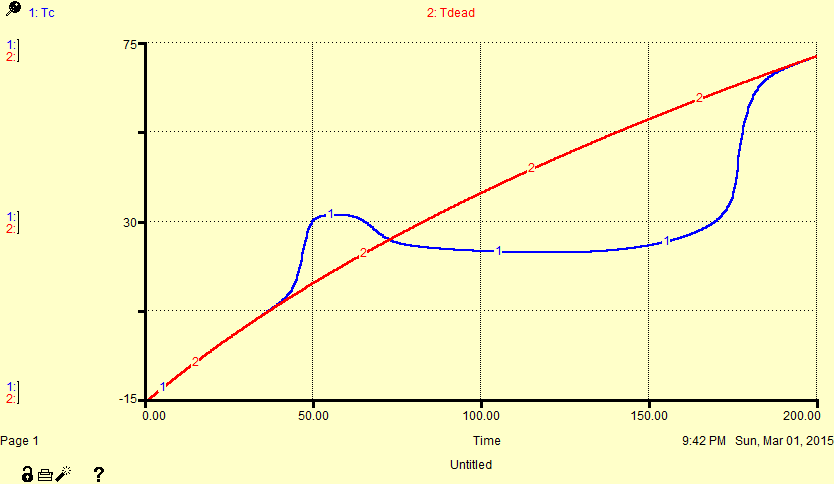
\includegraphics[width=0.9\textwidth]{./p1.jpg}
\end{figure}
\begin{itemize}
\item Black daisies cause planet to warm up and make it more habitable early on
\item White daises keep the planet cool and greatly extend the planet's life span
\end{itemize}
}

\frame{
\frametitle{1. Initial simulations}
\begin{figure}
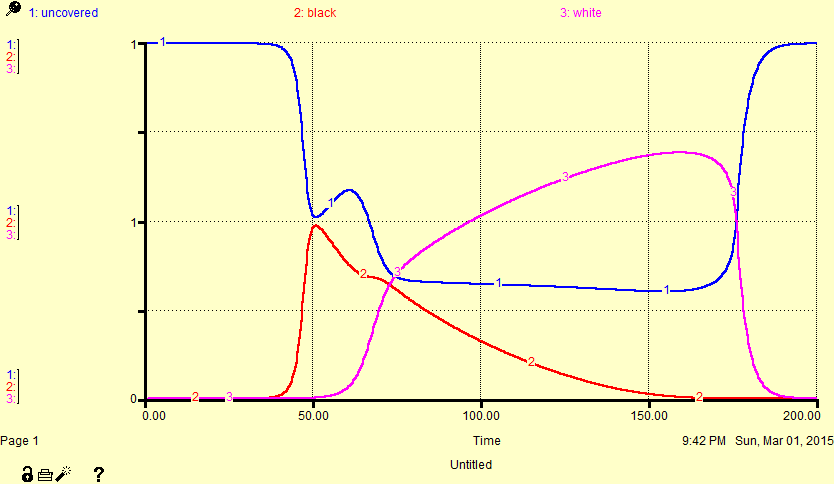
\includegraphics[width=0.9\textwidth]{./p1b.jpg}
\end{figure}
\begin{itemize}
\item Black daisies grow rapidly (unstable growth), and then gradually die off
\item White daisies grow slowly, then rapidly die off
\end{itemize}
}

\frame{
\frametitle{2. Varying the daisy albedos}
\begin{figure}
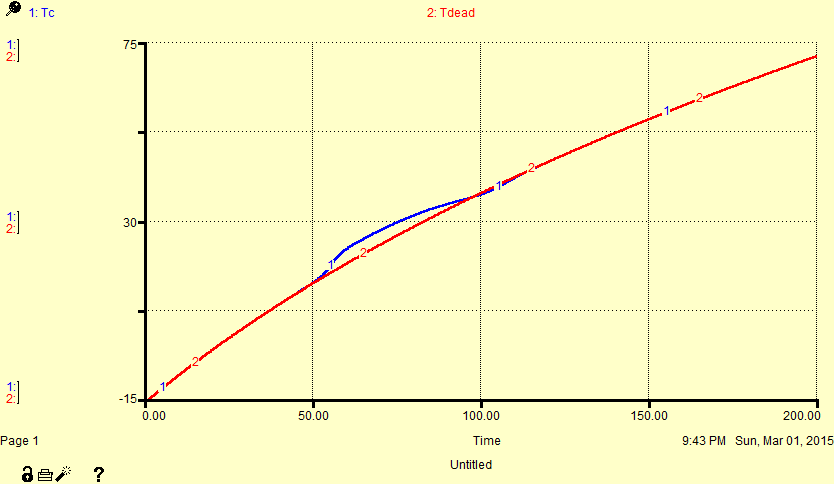
\includegraphics[width=0.9\textwidth]{./p2a.jpg}
\end{figure}
\begin{itemize}
\item Black albedo = 0.4; white albedo = 0.6
\item Moderate albedos $\Rightarrow$ reduced lifespan
\end{itemize}
}

\frame{
\frametitle{2. Varying the daisy albedos}
\begin{figure}
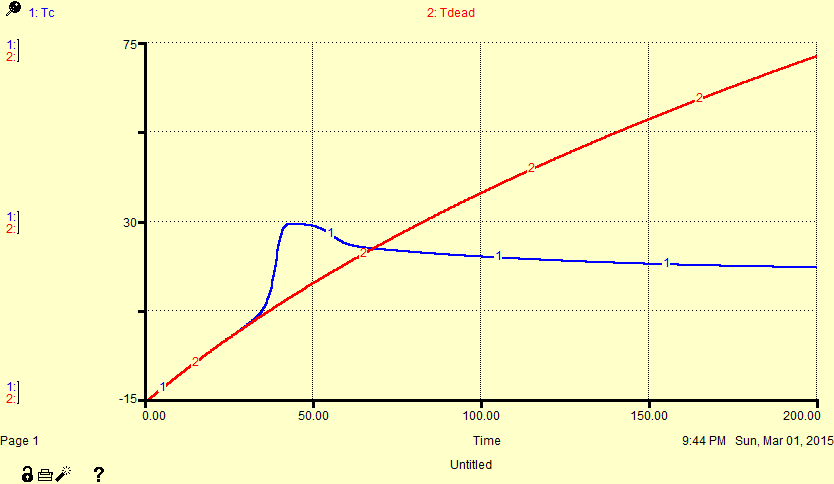
\includegraphics[width=0.9\textwidth]{./p2b.jpg}
\end{figure}
\begin{itemize}
\item Black albedo = 0.05; white albedo = 0.95
\item Extreme albedos $\Rightarrow$ increased lifespan
\end{itemize}
}

\frame{
\frametitle{3. Varying the growth curves}
\begin{figure}
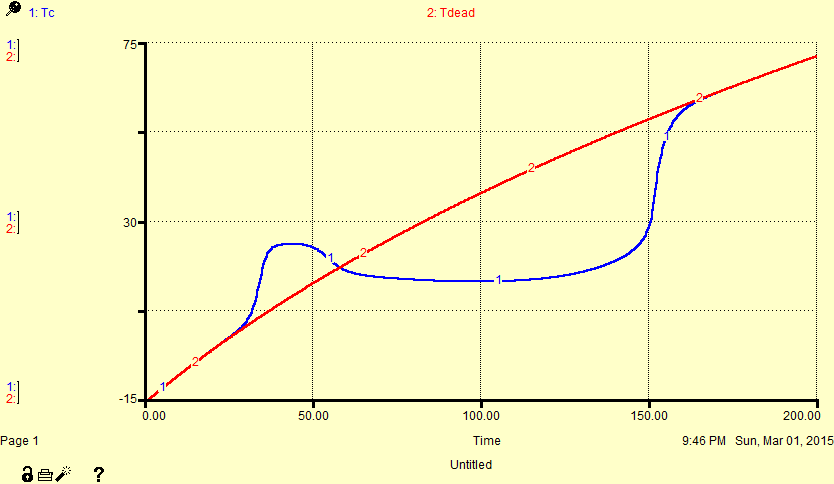
\includegraphics[width=0.9\textwidth]{./p3a.jpg}
\end{figure}
\begin{itemize}
\item Reduce optimal temperature for daisy growth
\item Planet becomes habitable sooner, but daisies also die off sooner
\end{itemize}
}

\frame{
\frametitle{3. Varying the growth curves}
\begin{figure}
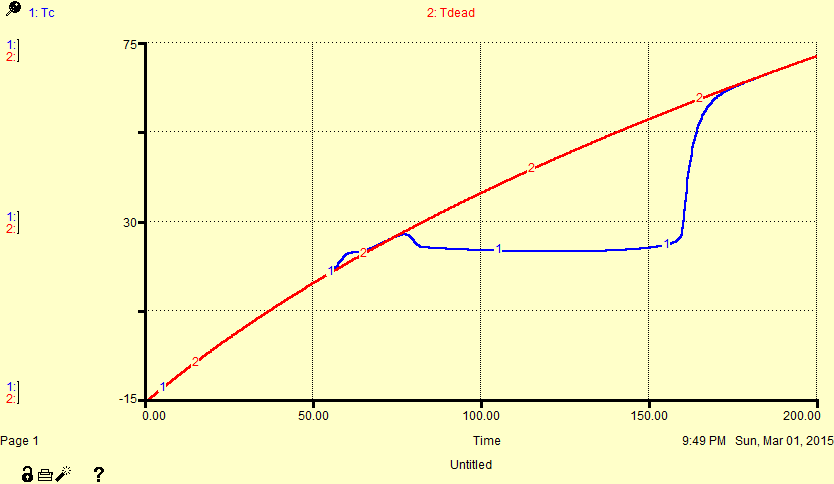
\includegraphics[width=0.9\textwidth]{./p3b.jpg}
\end{figure}
\begin{itemize}
\item Reduce temperature range over which daisies survive
\item Feedbacks weaker, and planet lifespan is reduced
\end{itemize}
}

\frame{
\frametitle{4. Plagues}
\begin{figure}
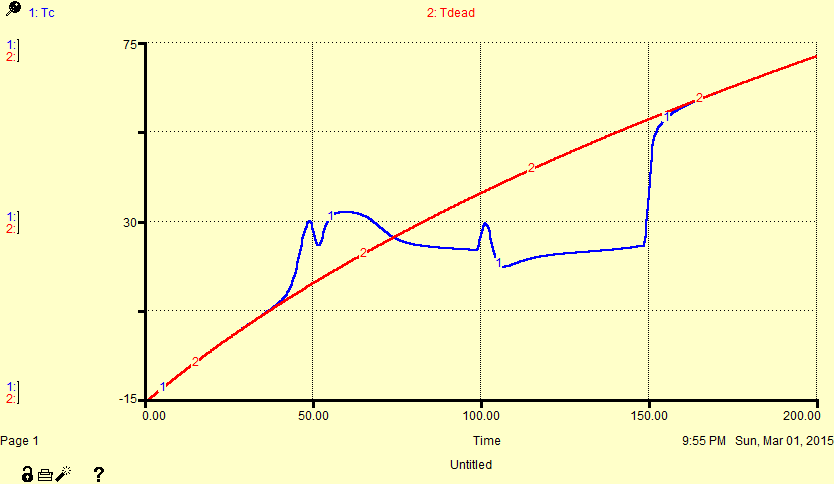
\includegraphics[width=0.9\textwidth]{./p4a.jpg}
\end{figure}
\begin{itemize}
\item Had 3 similar plagues
\item System recovered from the first two, but third one led to rapid extinction
\end{itemize}
}

\frame{
\frametitle{4. Plagues}
\begin{figure}
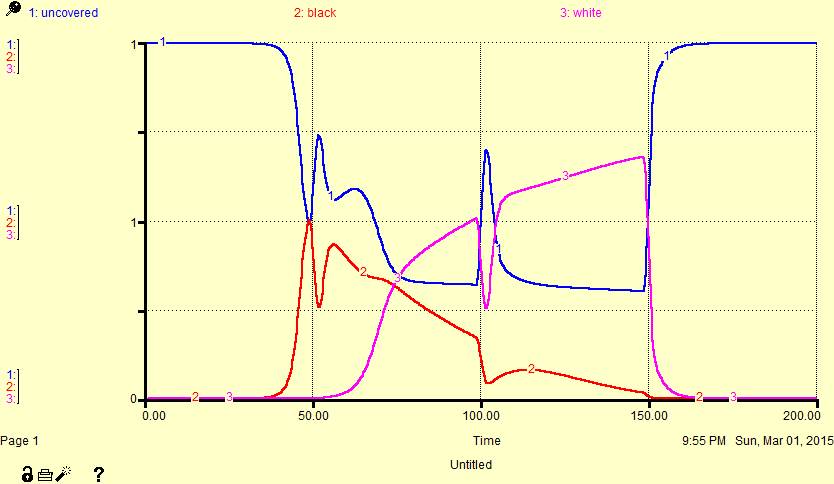
\includegraphics[width=0.9\textwidth]{./p4b.jpg}
\end{figure}
}

\frame{
\frametitle{5. Volcanic eruption}
\begin{figure}
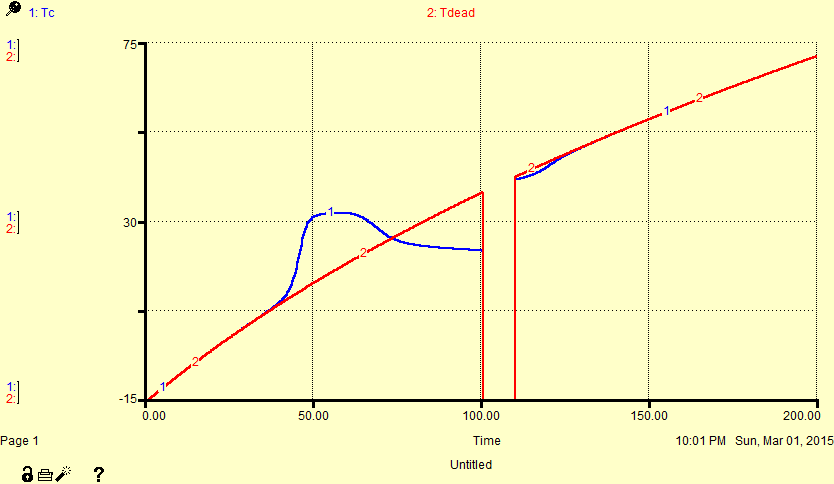
\includegraphics[width=0.9\textwidth]{./p5.jpg}
\end{figure}
\begin{itemize}
\item Larger perturbation than plagues
\item Occurs at same time as second plague, but system is unable to recover
\end{itemize}
}

\end{document}
